%===========================================================================
%	II.4 Progressive Web Apps (PWAs)
%===========================================================================

Dieses Unterkapitel erklärt die bereits erwähnte \acf{pwa} und nennt Kriterien, die von ihr erfüllt werden. Anschließend folgen die verwendeten Frameworks für die Entwicklung der \ac{pwa}. Ein Überblick über diese ist essenziell für das Verständnis von Kapitel \ref{chap:implementierung}, in welchem die spezifischen Implementierungsschritte betrachtet werden.

Eine \acf{pwa} ist ein nächster Schritt nach der Dynamisierung statischer \acsu{html}-Seiten durch JavaScript und Front-End-Frameworks. Der Software-Entwickler und Autor \textsc{Majid Hajian} charakterisiert \ac{pwa}s mit acht Eigenschaften. Die wichtigsten dieser Charakteristiken werden im Folgenden zusammenfassend erläutert:

% - DESCRIPTION ----------------------------------------------------------------
\begin{description}
	\item[Installierbarkeit]
	Der Nutzer einer Webanwendung kann diese lokal auf seinem Gerät installieren. Sie kann anschließend, wie eine native App, vom Startbildschirm aus gestartet werden. Um die Webanwendung zu nutzen muss ein Nutzer nun keinen Zwischenschritt mehr über den Browser tätigen.
  
	\item[Ähnlichkeit mit einer nativ implementierten App]  
	Klassischerweise werden Android-Apps in Java bzw. neuerdings Kotlin und iOS-Apps in Swift programmiert. Die \ac{pwa} soll, wie eine native App, auf die Hardware des Mobilgerätes zugreifen können (beispielsweise für die Nutzung des Bluetooth-Chips). Außerdem unterscheidet sich das \ac{ui} der \ac{pwa} nicht maßgeblich von der nativen App. 
  
	\item[Offline-Verwendung] 
	Die \ac{pwa} soll unabhängig von einer Netzwerkverbindung funktionieren. Sie ist nach dem \textit{Offline-First}-Design konzipiert. Die Google-Chrome Dokumentation für Cloud-Entwickler beschreibt Offline-First-Apps als Webanwendungen, deren Dateien (\acs{html}, \acsu{css}, JavaScript etc.) bereits heruntergeladen sind. Daten werden temporär über eine Browser-Schnittstelle gespeichert und bei Bedarf synchronisiert. Außerdem kann die Anwendung auf eine unterbrochene Netzwerkverbindung reagieren \cite{GoogleOfflineApps}. Die \ac{pwa} ist demnach eine Webanwendung, die sowohl online, als auch offline nutzbar ist.

	\item[Optimierung für Mobilgeräte]  
  	Die \ac{pwa} ist für die (meist leistungsschwache) Mobilhardware konzipiert und funktioniert hierauf ohne Performanzprobleme. \textsc{Hajian} legt besonders auf das schnelle Laden beim Start der Anwendung wert.
  	
  	\item[Informierung des Nutzers] 
  	Wie native Apps kann die \ac{pwa} den Nutzer über Push-Nachrichten informieren oder zur Interaktion auffordern \cite[S. 1f.]{Hajian2019}.
\end{description}
% ------------------------------------------------------------------------------

Diese Charakteristika decken sich mit der Beschreibung durch die Entwicklerdokumentation der \ac{pwa} von Google. Im Vergleich zu \textsc{Hajian} ist diese etwas spezifischer und erwähnt bspw. die Kontrolle des Anwendungs-Caches durch einen JavaScript-Service-Worker (siehe Abs. \ref{sub:service_worker}), um die Abhängigkeit von einer Netzwerkverbindung aufzuheben.
\cite{GooglePWAOverview}



% = II.4.1 Installation einer PWA ================================================================
\subsection{Installation einer \acf{pwa}}
Diese Arbeit betrachtet die \ac{pwa}, da sie (wie auch eine native Anwendung) lokal auf einem Gerät installiert werden kann. Es ist dafür kein zentraler Bezugspunkt nötig; die Installation wird über den Browser gestartet. Die Aufforderung zur Installation einer \ac{pwa} kann entweder über den Browser (siehe Abb. \ref{fig:pwainstallationprompt}) oder über ein Element der Website erfolgen, dass ein Event erzeugt, wie bspw. einen Button oder einen Dialog.

% - FIGURE ----------------------------------------------------------------
\begin{figure}[h!]
	\centering
	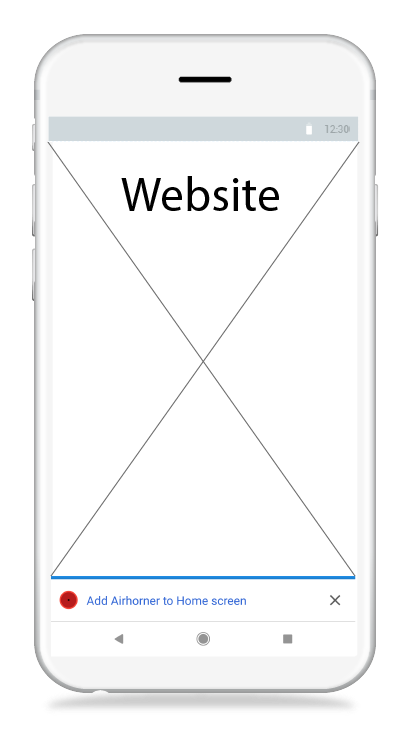
\includegraphics[width=0.5\linewidth]{img/fig/2-4-1_Install_PWA_Wireframe}
	\caption{Browserdialog zur Installation einer \ac{pwa} \cite{PWAAddToHomeScreenPrompt}}
	\label{fig:pwainstallationprompt}
\end{figure}
% -------------------------------------------------------------------------

\newpage
 

Zwar bezeichnen Browser die Installation meist nur mit der Aufschrift \textit{Zum Startbildschirm hinzufügen}, tatsächlich generiert der Browser aber dann eine WebAPK, welche auf dem Gerät installiert wird. Auf Desktopgeräten startet die \ac{pwa} in einem eigenen, stark verschlankten Browserfenster ohne Suchleiste und Bedienelemente. \cite{GooglePWAInstallation}

% ==============================================================================================



% = II.4.2 Manifestdatei =======================================================================
\subsection{Manifest-Datei für die Konfiguration der \ac{pwa}}
Um die \ac{pwa} auf einem Gerät installieren zu können, muss ein sog. \textit{Web-App-Manifest} zur Verfügung gestellt werden. Dieses ist eine \ac{json}-Datei, welche Konfigurationsparameter für die Anwendung enthält. \cite{GooglePWAManifest}

% - SOURCE CODE ----------------------------------------------------------------
\begin{listing}[H]
    \inputminted{json}{src/2-1_manifest_sample.json}
    \caption{Manifest-Datei einer \ac{pwa}}
      \label{sourcecode:manifest_sample}
\end{listing}
% ------------------------------------------------------------------------------

Quellcode-Auschnitt \ref{sourcecode:manifest_sample} zeigt den Inhalt einer Manifest-Datei. Neben diversen Icons (Zz. 4-15) werden auch \textit{Name} (Z. 3), \textit{Farbschema} (Z. 20) und \textit{Anzeigeeinstellungen} (Z. 18) festgelegt.
Die Manifest-Datei wird im \acs{html} der Webanwendung eingebunden, siehe Quellcode-Ausschnitt \ref{sourcecode:manifest_include}. 

% - SOURCE CODE ----------------------------------------------------------------
\begin{listing}[h!]
    \inputminted{xml}{src/2-2_include_manifest.html}
    \caption{Einbinden der Manifest-Datei}
      \label{sourcecode:manifest_include}
              %https://developers.google.com/web/fundamentals/web-app-manifest?hl=en
\end{listing}
% ------------------------------------------------------------------------------

Es ist die Einfachheit dieses Prozesses hervorzuheben: Das Hinzufügen einer (wenige Zeilen langer) \ac{json}-Datei macht die gesamte Webanwendung installierbar. Es wird kein App-Store, manueller Dateidownload oder Installer benötigt.
%
% ==============================================================================================



% = II.4.3 Service Worker =======================================================================
\subsection{Service Worker für Offline-Funktionalität und Benachrichtigungen}
\label{sub:service_worker}

Damit die \ac{pwa} trotz fehlender Netzwerkverbindung funktioniert, wird ein besonderer Mechanismus benötigt: Der sog. \textit{Service-Worker}. Mit ihm können Abhängigkeiten der App lokal gecacht werden, sodass die Anwendung auch bei schlechter oder gar fehlender Netzwerkverbindung funktioniert \cite[S. 7]{BeginningPWA}.

Ein Service-Worker ist ein vom \ac{ui} separiert laufendes Hintergrundskript der Webanwendung (s. Abb. \ref{fig:serviceWorker}). Er wird genutzt, um Bilder, Skripts, Styles oder ganze Seiten zu cachen. Bei bestehender Netzwerkverbindung führt er nötige Synchronisierungen durch. Nicht zuletzt ist er auch für das Senden von Push-Benachrichtigungen zuständig \cite[S. 24]{BeginningPWA}.
%
% - FIGURE ----------------------------------------------------------------
\begin{figure}[h!]
        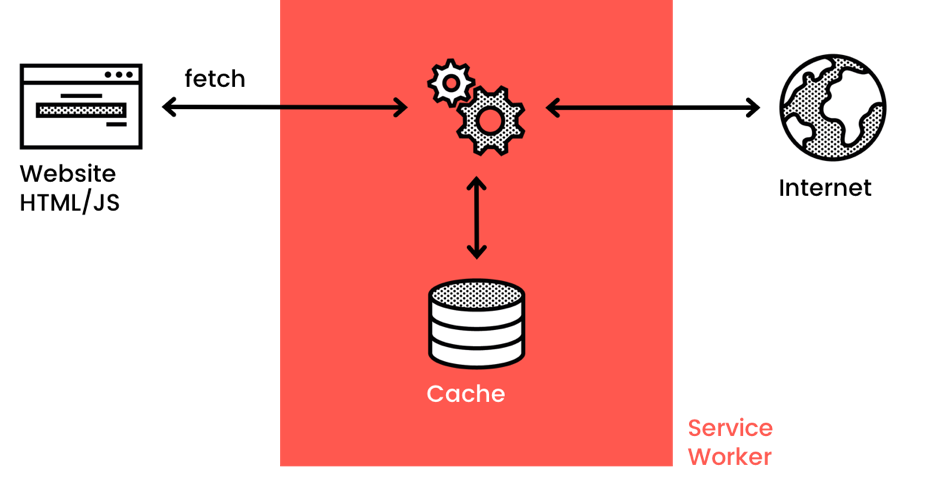
\includegraphics[width=\linewidth]{img/fig/2-4-2_Service_Worker_Concept.png}
        \centering
        \caption{Konzept des Service Workers \cite{ServiceWorkerDiagramm}}
        \label{fig:serviceWorker}
\end{figure}
% -------------------------------------------------------------------------
%

Alle verbreiteten Desktop-Browser wie Google Chrome, Mozilla Firefox, Opera, Microsoft Edge und mittlerweile auch Apple Safari unterstützen das Service-Worker-Konzept. Der mobile Chrome-Browser unter Android unterstützt Service-Worker bereits vollständig, während Safari unter iOS noch an diesem Feature arbeitet. \cite[S. 9]{BeginningPWA}
%
% =============================================================================================



% = II.4.4 Plattformen =======================================================================
\subsection{\ac{pwa}-unterstützende Plattformen}
Das Projekt \textit{CanIUse} aggregiert Daten zu Webstandards des W3-Konsortiums sowie zu Browser-Dokumentationen. Es wird als Quelle für die Unterstützung von Features durch aktuelle Browser herangezogen.

Apples mobiler Browser Safari unterstützt eines der wichtigsten Features der \ac{pwa} noch nicht vollständig; es fehlen Teile des Web-App-Manifests. Allerdings wird der Service-Worker vollständig unterstützt \cite{CanIUseWebManifest}. Wann und ob Safari die Unterstützung für das Manifest implementiert, ist unklar und bleibt abzuwarten. Die aktuelle Teilunterstützung lässt jedoch vermuten, dass sich Apple nicht grundsätzlich gegen die \ac{pwa} weigert.
 %Die Versionen zeigen aber eine stetig voranschreitende Integration der, erweitert den Funktionsumfang in den neusten Versionen von iOS. 
% https://medium.com/@firt/progressive-web-apps-on-ios-are-here-d00430dee3a7
% Source: https://developers.google.com/web/progressive-web-apps/desktop
Die Nutzung von \ac{pwa}s ist nicht ausschließlich auf Smartphones begrenzt. Wie \textit{normale} Desktop-Programme werden Desktop-\acp{pwa} in einem eigenen Fenster gestartet. 
Der Unterschied zwischen den Bedienelementen nativer Desktop-Anwendungen und Desktop-\acp{pwa} ist ausschließlich farblicher Natur. Stark vereinfacht beschrieben sind Desktop-\acp{pwa} Browserfenster ohne Tabs und Adressleiste. Durch die Nutzung von Service-Workern, welche die Webanwendung cachen, sind auch Desktop-\acp{pwa} nicht von einer Netzwerkverbindung abhängig.

Grundsätzlich können Desktop-\acp{pwa} auf jedem Betriebssystem installiert werden, auf welchem auch Google Chrome (Version größer 73) installiert werden kann: Windows, Mac, Linux und Chrome OS.
\cite{GooglePWADesktop}
%
%============================================================================================



% = II.4.5 JavaScript =======================================================================
\subsection{Grundlage der Webanwendung: JavaScript-Laufzeitumgebung \textit{Node.js}}

%NodeJSWebsiteAbout
\textit{Node.js} ist eine open-source JavaScript-Laufzeitumgebung für die Entwicklung skalierbarer Webanwendungen 
\cite{NodeJSWebsiteAbout}.
Selbst baut Node.js auf der \textit{V8-Engine} auf, einer Laufzeitumgebung, die auch von Google Chrome genutzt wird 
%NodeJSRecepies
\cite[S. 1]{NodeJSRecepies}.
% PracitalNodeJS
Wegen zeitsparenden Features, wie automatischem Typecasting oder der Tatsache, dass Node.js alle Daten als Objekt behandelt, erfreut sich Node.js großer Beliebtheit 
\cite[S. 12]{PracitalNodeJS}.
Die Kombination mit dem \textit{Package Manager} \texttt{npm} ermöglicht die einfache Installation und Nutzung von Modulen, um die Funktionalität der Plattform zu erweitern. 
\cite[S. 9]{NodeJSRecepies}.
%
% ===========================================================================================



% = II.4.6 Angular =======================================================================
\subsection{Front-End-Framework \textit{Angular} für die Entwicklung von Webanwendungen}
\textit{Angular} ist ein open-source TypeScript-basiertes Framework zur Entwicklung von Webanwendungen, welches Node.js nutzt.
%https://octoverse.github.com/projects
Mit über Achttausend bzw. über Siebentausend mitwirkenden Entwicklern belegen das Angular \ac{cli} resp. das Angular-Framework die Plätze 4 und 6 der größten Projekte auf GitHub. 
% https://octoverse.github.com/projects
\cite{OctoverseGitHubStatistics}

Das Framework arbeitet auf Basis von Komponenten. Ein Eingabefeld, eine Seite oder eine Liste werden in Angular als separate Komponenten betrachtet. Auch in der Dateistruktur werden Komponenten stark getrennt. Jede Komponente besitzt bspw. ein eigenes \acs{css}- (oder \acsu{scss}) und HTML-File. Eine Komponente für eine Seite kann so auch eine oder sogar mehrere Listenkomponenten einbinden. Durch die Wiederverwendung von Quellcode-Fragmenten in Komponenten wird der Programmquellcode sehr übersichtlich und strukturiert.

% - FIGURE ----------------------------------------------------------------
\begin{figure}[h!]
	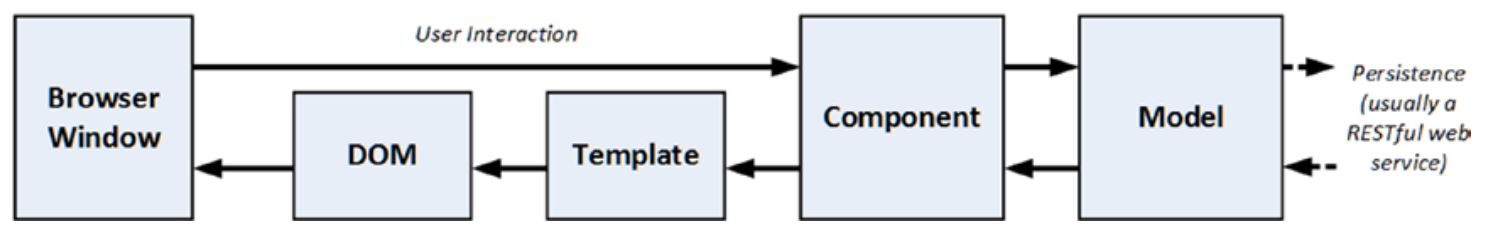
\includegraphics[width=\linewidth]{img/fig/2-4-3_Angular_MVC_Concept.jpg}
	\centering
	\caption{MVC Konzept von Angular \cite[S. 35, Abbildung 3-4]{ProAngular}}
	\label{fig:angularmvc}
\end{figure}
% -------------------------------------------------------------------------
\newpage
Eine Angular-Anwendung ist wie folgt in drei Einheiten gegliedert:

\begin{description}
	\item[Model] enthält Logik für die Verwaltung von Daten, bspw. das Erstellen, Speichern oder Modifizieren. Dies kann über die Kommunikation mit einem Webserver via \acs{rest}-\acsu{api} erfolgen. Das Model enthält keine Logik, um mit dem Nutzer zu interagieren.
	\item[Component] enthält Logik für das Aktualisieren der Daten im Model aufgrund Nutzerinteraktion.
	\item[Template] enthält Logik und Markup, um dem Nutzer Daten anzeigen zu können \cite{ProAngular}.
\end{description}

%
% ===========================================================================================
